\documentclass[10pt,a4paper]{article}
\usepackage{fontspec,polyglossia}
\setmainlanguage{russian}
\setmainfont{Times New Roman}
\usepackage{amsmath,amssymb,booktabs,tabularx,graphicx}
\usepackage[margin=17mm]{geometry}
\usepackage[hidelinks]{hyperref}
\usepackage{titlesec}
\titleformat{\section}{\large\bfseries}{}{0pt}{}
\titlespacing*{\section}{0pt}{8pt}{4pt}
\setlength{\parindent}{0pt}
\setlength{\parskip}{4pt}
\setlength{\emergencystretch}{3em}
\begin{document}
{\Large\bfseries Практическая проверка MG для выбора RL-политики}\par\medskip

\section*{Идея}

В RL часто нужно выбрать чекпоинт политики до deployment. Номинальная награда на обычной симуляции может не отражать устойчивость к изменению условий исполнения. Здесь проверяется, может ли MG по короткому scalar action log выбрать политику, которая лучше переносится на скрыто изменённую динамику привода.

Это offline evaluation уже обученных политик Walker2d. Нового обучения в этом эксперименте нет, поэтому результат показывает пользу метода для выбора и мониторинга политик, но не sample efficiency обучения.

\section*{Постановка}

Seed 231 использован как development pilot; итоговая таблица использует только четыре confirmation seed 232--235. Для каждого seed доступны 16 кандидатов:

\begin{itemize}
\item четыре коэффициента action smoothing: (0, 0.25, 1, 4);
\item четыре чекпоинта: (262144, 524288, 786432, 1048576) шагов.
\end{itemize}

Исходные политики обучались PPO управлять шестью приводами Walker2d. Штраф добавлялся к PPO-loss за квадрат разности средних команд на соседних состояниях; команда при исполнении не фильтровалась. Все ветки начинались с одного общего навыка. Здесь проверяется перенос этих уже обученных политик, а не способность обучиться с нуля.

На трёх номинальных rollout выбирался кандидат по одному из методов: MG, spectral entropy, normalized increments, scalar recurrence, J1, номинальная reward и фиксированный pilot baseline. Кандидаты с менее чем двумя полными rollout или reward ниже 90\% от лучшего номинального кандидата исключались. Один rollout содержит 256 шагов разогрева и 2048 шагов измерения; управляющий шаг составляет 0.008 с. Падения на разогреве дают нулевой итоговый reward.

MG анализирует норму вектора из шести команд: окно 2048, E=20, задержка 8, k=20, Theiler exclusion 312, dither seed 123. Минимизируется медиана MG по полным номинальным эпизодам. Остальные scalar методы используют тот же лог: entropy --- энтропию спектра, increments --- квадрат приращений, нормированный на удвоенную дисперсию, recurrence --- минимальную нормированную ошибку возврата по лагам 20--250. J1 использует все шесть команд. Номинальная reward усредняет все эпизоды, включая падения. Fixed pilot всегда выбирает коэффициент 0.25 и финальный чекпоинт, если он проходит общий фильтр.

После выбора политика тестировалась на пяти новых reset при шести скрытых условиях: мягкое запаздывание привода (alphain{0.05,0.1,0.2}) и action noise (sigmain{0,0.02}). Исполнительная команда имела вид

\[
a_t^{\mathrm{exec}}=(1-\alpha)u_t+\alpha a_{t-1}+\varepsilon_t.
\]

В формуле $u_t$ --- команда политики, а $a_t^{\mathrm{exec}}$ --- внутреннее состояние привода; в среду передаётся его обрезанная до [-1,1] версия. Запаздывание и шум действуют также на разогреве; это дополнительный проверенный сдвиг относительно первого эксперимента. Основная метрика --- сумма reward за измерительные шаги, делённая на фиксированные 2048; после падения остаток нулевой. Дополнительно считается доля полных эпизодов. На seed и выбранного кандидата приходится 6 условий по 5 reset, то есть 30 эпизодов. Повторы reset не заменяют независимые seed.

\section*{Результаты}

\begin{center}\small
\begin{tabularx}{\linewidth}{l>{\raggedright\arraybackslash}X>{\raggedright\arraybackslash}X>{\raggedright\arraybackslash}X}
\toprule
Selector & Target reward & Complete episodes & Regret to oracle \\
\midrule
MG & \textbf{4.313} & 90.8\% & 0.359 \\
Spectral entropy & \textbf{4.480} & \textbf{97.5\%} & \textbf{0.191} \\
Scalar recurrence & 4.398 & 95.0\% & 0.273 \\
Fixed pilot & 4.310 & 90.8\% & 0.361 \\
Nominal reward & 4.005 & 80.0\% & 0.667 \\
Random eligible & 4.286 & 90.9\% & 0.385 \\
J1 & 2.999 & 47.5\% & 1.672 \\
Normalized increments & 3.064 & 49.2\% & 1.608 \\
Oracle & 4.671 & 100\% & 0 \\
\bottomrule\end{tabularx}\end{center}

В этом измерении MG улучшает выбор относительно nominal reward на 0.308 reward, то есть примерно на 7.7\%, и повышает долю полных эпизодов с 80.0\% до 90.8\%. Относительно J1 и normalized increments выигрыш существенно больше. Oracle имеет доступ к целевым результатам, остальные методы --- только к номинальным. Random eligible --- математическое ожидание равномерного выбора среди допустимых кандидатов, без случайного удачного запуска.

MG не превосходит spectral entropy и уступает scalar recurrence по средней survival rate. Разница с fixed pilot практически отсутствует. При четырёх confirmation seeds sign-flip tests не дают статистически убедительного превосходства MG над отдельными baseline: это полезный exploratory результат, а не доказательство универсального превосходства.

\begin{center}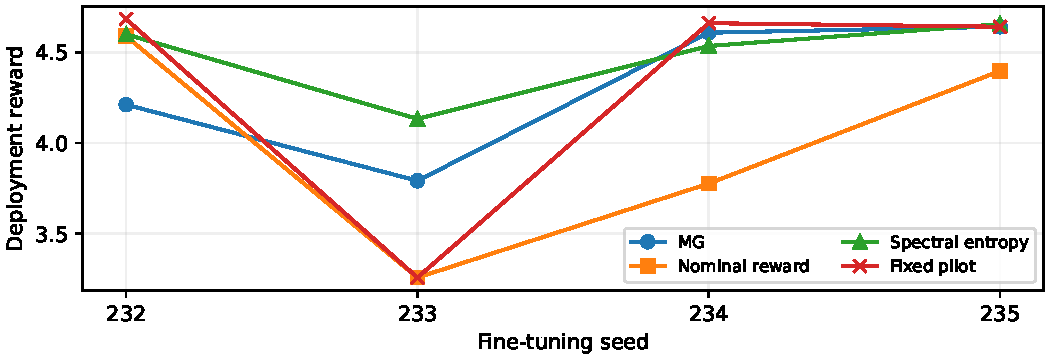
\includegraphics[width=\linewidth,height=.30\textheight,keepaspectratio]{selection_results.pdf}\end{center}

\section*{Стоимость}

На одном CPU с одним потоком измерение MG по одному action log занимает около 0.516 с. Spectral entropy занимает 0.00014 с, increments --- 0.00003 с, J1 --- 0.00004 с, recurrence --- 0.0062 с. Поэтому преимущество MG здесь выражается в качестве выбора относительно reward и J1, а не в скорости обработки scalar log.

Проверка 30 целевых эпизодов на одного кандидата занимает около 44.7 с; три номинальных эпизода --- 5.52 с. Вместе с тремя расчётами MG получается оценка 7.06 с против 44.7 с, то есть примерно в 6.3 раза дешевле полного целевого теста. Это расчёт по медианным компонентам на одной выбранной политике; качество решения различается. Энтропия использует те же номинальные эпизоды и почти не добавляет вычислений. Расход обучения кандидатов общий и сюда не включён; экономия обучения или ускорение curriculum не измерялись. Замеры выполнялись последовательно после параллельных тестов: Intel i5-12500H, CPU, один поток, три повтора rollout и семь повторов признаков.

\section*{Контроль первого варианта}

Первый эксперимент выбирал среди четырёх финальных политик. После номинального разогрева включалась задержка 1, 2 или 3 полных управляющих шага; десять новых reset на каждую задержку. Pilot --- seed230, подтверждение --- 231--235. По итогам пяти seed MG получил reward 0.541 против 0.319 у reward-only, но лишь 2 из 150 выбранных эпизодов завершились без падения. MG на всех пяти seed выбрал коэффициент 1, совпав с фиксированным pilot baseline. Поэтому рост reward на 70\% здесь не означает практически пригодного управления. Результат сохранён как отрицательный stress test.

\section*{Вывод}

Есть описательный выигрыш MG над nominal reward, J1 и increments в новом целевом тесте. Но это слабое основание для главного результата статьи: лучшие дешёвые конкуренты сильнее, fixed pilot почти равен MG, а случайный допустимый выбор отстаёт лишь на 0.027 reward. Четыре confirmation seed происходят от одного навыка; данные прежних политик помогли выбрать гипотезу. Перед подтверждением второй протокол был зафиксирован, но seed231 разрабатывался итеративно. Упрощение лога не гарантирует освоение задачи, устойчивость тела или готовность к curriculum.

Он не подтверждает, что MG превосходит все аналоги. Spectral entropy показала лучший результат, а recurrence была конкурентоспособна. Поэтому наиболее честная формулировка для статьи:

\begin{quote}In this exploratory actuator-shift benchmark, MG-based checkpoint selection obtained higher mean deployment return than nominal-reward selection on four held-out fine-tuning seeds, but did not outperform spectral entropy or establish a benefit over the pilot-selected fixed configuration.\end{quote}

Для сильного результата я бы проверял MG как дополнительный сигнал, а не замену успеха задачи:

\begin{itemize}
\item \textbf{Curriculum для управления при возмущениях.} PPO сначала учит движение без внешних толчков, затем с ними. Переход разрешён при достаточном reward; MG определяет момент проверки готовности. Нужно заново обучить ветки с reward-only, фиксированным расписанием, learning progress, entropy и MG при равном числе взаимодействий. Критерий --- площадь под кривой success на конечной задаче; checkpoint replay её не доказывает.
\item \textbf{Предотвращение posterior collapse в текстовом VAE.} При изменении MG фиксированного reconstruction-log контроллер временно снижает KL-вес. Сравнить с KL/free-bits/cyclical schedule, периодическим контроллером и entropy при равном вычислительном бюджете. Критерий --- удержанная информация при сопоставимом reconstruction quality; scalar acquisition обязательно входит в стоимость.
\item \textbf{Остановка обучения рекуррентного генератора с дорогой сертификацией.} MG инициирует полносостоянийную проверку устойчивости и прекращение обучения только после её успеха. Сравнить с ошибкой выхода, recurrence, entropy и периодическими проверками; критерий --- полное время до заданного качества и устойчивости. Наиболее естественно связано с теорией, но может проиграть recurrence.
\end{itemize}

Эти три направления --- непроверенные следующие гипотезы. Текущие результаты не добавлялись в статью. Сейчас сохранены:

\begin{itemize}
\item `seed230.json` --- development pilot;
\item `checkpoint\_selection\_s231.csv` ... `checkpoint\_selection\_s235.csv` --- raw checkpoint evaluations;
\item `checkpoint\_selections.csv`, `checkpoint\_summary.csv` --- frozen selector results;
\item `audit.json` --- checks of coverage, target independence and replay;
\item `timing\_summary.csv` --- analysis costs;
\item `PROTOCOL.md` и `CHECKPOINT\_PROTOCOL.md` --- постановки и границы интерпретации.
\end{itemize}
\end{document}